
\section{Introduction}
Correlation clustering is one of the most prominent problems in clustering, 
as it cleanly models community detection problems~\cite{veldt2018, SDELM21} and provides a way to decompose complex network structures~\cite{Wirth17, mccallum2004conditional}. 
The input to the unweighted correlation clustering problem is a complete graph $G=(V,E)$, where $|V|=n$ and each edge $e \in E$ is labeled positive $(+)$ or negative $(-)$.  
If the edge $(u,v)$ is positive, this indicates that $u$ and $v$ are similar, 
and analogously if the edge $(u,v)$ is negative, this indicates that $u$ and $v$ are dissimilar. 
The output of the problem is a partition of the vertex set into parts $C_1, C_2, \ldots$, where each part represents a cluster.   

The output should cluster similar vertices together and separate dissimilar vertices.
Specifically, for a fixed clustering (i.e., partition of the vertices), a positive edge $(u, v)$ is a \emph{disagreement} with respect to the clustering if $u$ and $v$ are in different clusters and an \emph{agreement} if $u$ and $v$ are in the same cluster.
Similarly, a negative edge $(u,v)$ is a disagreement with respect to the clustering if $u$ and $v$ are in the same cluster 
and an agreement if $u$ and $v$ are in different clusters.  
The goal is to find a clustering that minimizes some objective
that is a function of the disagreements.\footnote{Note that the sizes and number of clusters are unspecified.}
For example, the most commonly studied objective minimizes the total number of disagreements.



As an easy example to illustrate the problem,
consider a social network. Every pair of people has an edge between them, 
and the edge is positive if the two people have ever met before, and negative otherwise.
The goal of correlation clustering translates to partitioning all the people into clusters so that people are in the same cluster as their friends/acquaintances and in different clusters than strangers. 
The difficulty in constructing a clustering is that the labels may not be consistent, making disagreements unavoidable. Consider in the social network what happens when there is one person with two friends who have never met each other ($u,v,w$ with $(u,v)$ and $(u,w)$ positive but $(v,w)$ negative).
The choice of objective matters in determining the best clustering.


For a given clustering $\mathcal{C}$, let $y_{\mathcal{C}}(u)$ denote the number of edges incident to $u$ that are disagreements with respect to $\mathcal{C}$ (we drop $\mathcal{C}$ and write $y$ when it is clear from context).  
The most commonly considered objectives are ${\lVert y_{\mathcal{C}} \rVert}_p = \sqrt[p]{\sum_{u \in V} y_{\mathcal{C}}(u)^p}$ for $p \in \mathbb{R}_{\geq 1} \cup \{\infty\}$,
the $\ell_p$-norms of the \emph{disagreement vector} $y$.   
Note that the optimal objective values may drastically vary for different norms too.  (For instance, in the example in Appendix A of \cite{PM16}, $V=A \sqcup B$\footnote{$\sqcup$ denotes disjoint union.}, where $|A| = |B| = n/2$, and all edges are positive except for a negative matching between $A$ and $B$. The optimal $\ell_\infty$-norm objective value is 1 whereas the optimal for $\ell_1$ is $\Theta(n)$.)
When $p=1$, this objective minimizes the total number of disagreements.  Setting $p = \infty$ minimizes the maximum number of disagreements incident to any node, ensuring a type of worst-case fairness.\footnote{In the social network example, minimizing the $\ell_1$-norm corresponds to finding a clustering that minimizes the total number of friends who are separated plus the total number of strangers who are in the same cluster. The $\ell_\infty$-norm corresponds to finding a clustering minimizing the number of friends any person is separated from plus the number of strangers in that person's same cluster.}  
Balancing these two extremes---average welfare on one hand and fairness on the other---is the $\ell_2$-norm, which minimizes the variance of the disagreements at each node.


Correlation clustering was proposed by Bansal, Blum, and Chawla \citeyearpar{BBC04} with the objective of minimizing the $\ell_1$-norm of the disagreement vector.
The problem is \textsf{NP}-hard and several approximation algorithms have been proposed \cite{BBC04, ACN-pivot, chawla2015near, cohen2022correlation}.  
Puleo and Milenkovic \citeyearpar{PM16} proposed studying $\ell_p$-norms of the disagreement vector for $p >1$, and they give a $48$-approximation for any fixed $p$. 
Charikar, Gupta, and Schwartz \citeyearpar{CGS17} introduced an improved $7$-approximation, which  Kalhan,  Makarychev, and  Zhou \citeyearpar{KMZ19} further improved to a $5$-approximation. When $p >1$, up until recently, the only strategies were LP or SDP rounding, and it has been of interest to develop fast combinatorial algorithms \cite{veldt2022correlation}.   
Davies, Moseley, and Newman \citeyearpar{DMN23} introduced a combinatorial $O(1)$-approximation algorithm for $p= \infty$ (see also \cite{minmax4approx} for a different combinatorial algorithm),
and leave open the question of discovering a combinatorial $O(1)$-approximation algorithm for $1 < p < \infty$.

 
In all prior work, solutions obtained for $\ell_p$-norms are tailored to each norm (i.e., $p$ is part of the input to the algorithm), and 
it was not well-understood what the trade-offs were between solutions
that optimize different norms.  
Solutions naively optimizing one norm can be arbitrarily bad for other norms (see Figure \ref{fig: star}). 
A natural question is whether this loss from using a solution to one objective for another is avoidable. 
More specifically:



\begin{figure}
    \centering
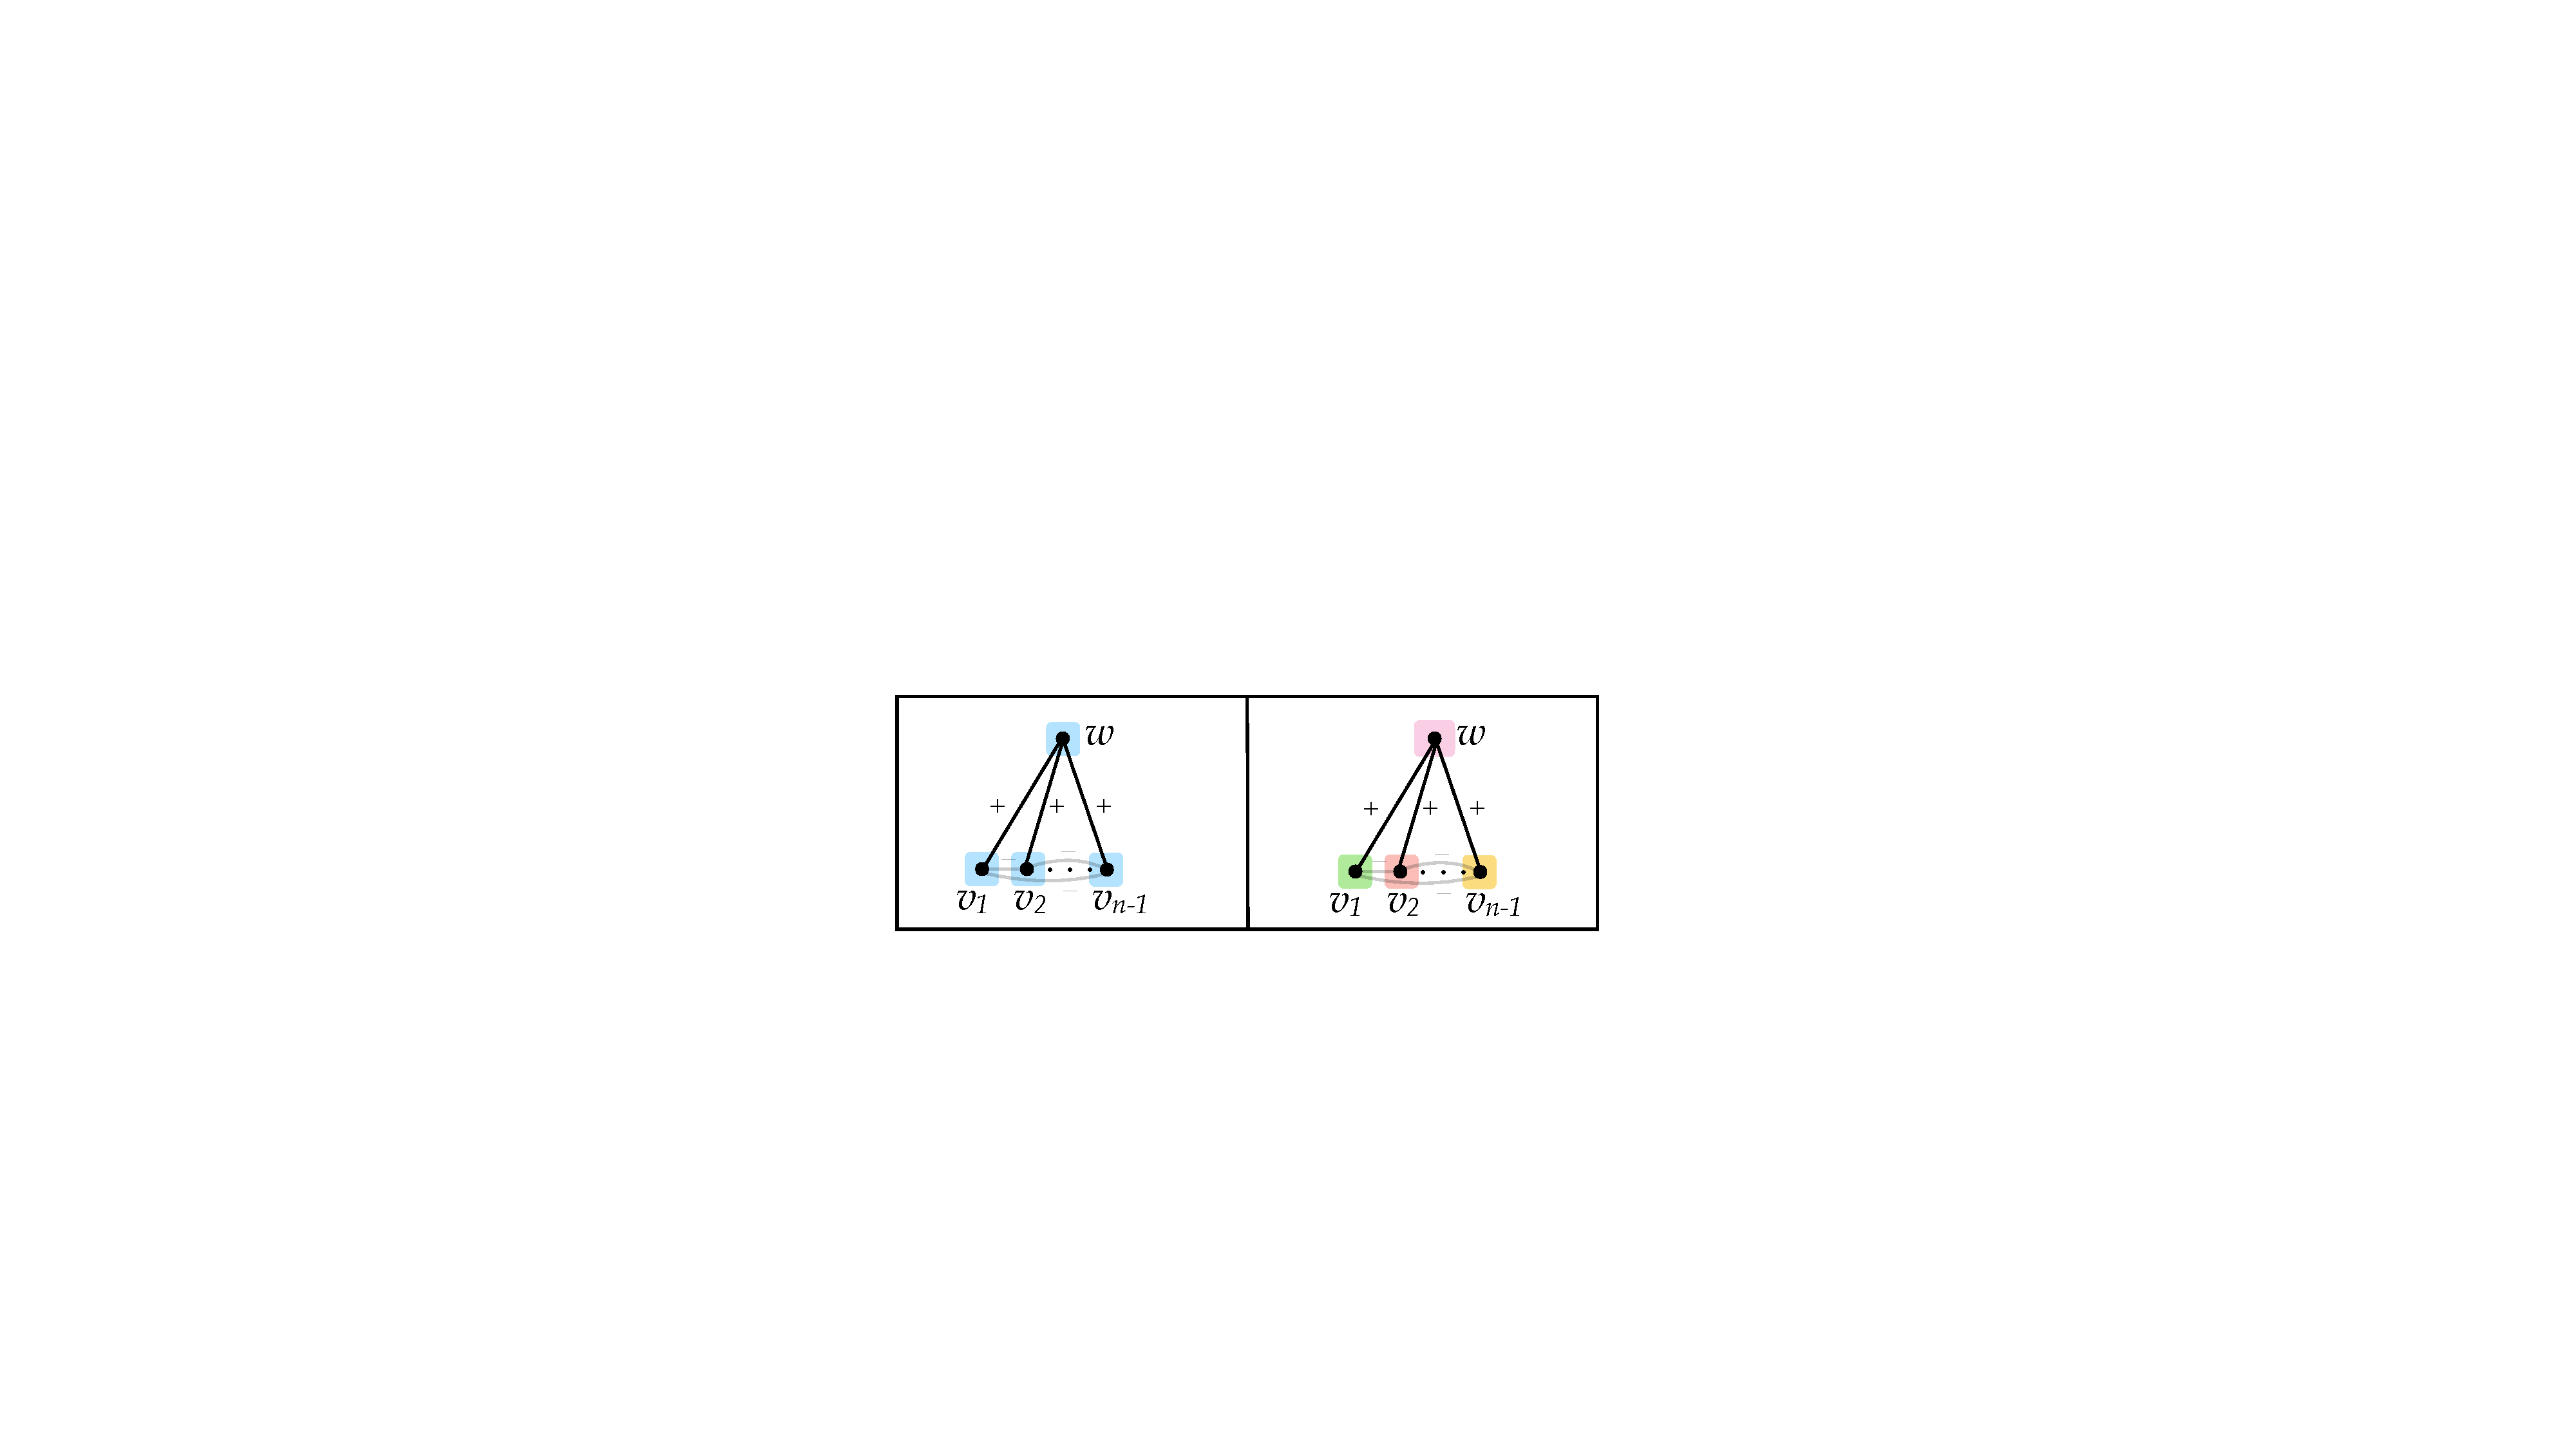
\includegraphics[width = 8cm]{soda-cc-figs-star.pdf}
    \caption{Two clusterings of the star graph, which has one node ($w$) with positive edges to all nodes, and the rest of the edges negative. \textbf{Left: }Clustering assigns all nodes to one (blue) cluster, and is (almost) optimal for the $\ell_\infty$-norm with cost $\Theta(n)$. 
    \textbf{Right: }Clustering assigns all nodes to different clusters and is (almost) optimal for the $\ell_1$-norm with cost $\Theta(n)$. The left solution is terrible for the $\ell_1$-norm, as the negative clique has $\Theta(n^2)$ edges that are disagreements. }
    \label{fig: star}
\end{figure}


\begin{center}
\emph{For any graph input to unweighted, complete correlation clustering,
does there exist a partition (clustering) that is \textbf{simultaneously} $O(1)$-approximate for all $\ell_p$-norm objectives?}
\end{center}


 Phrased another way, does there exist a \emph{universal algorithm} for $\ell_p$-norm correlation clustering---one which is guaranteed to produce a solution that well-approximates many objectives at once?
When the goal is to simultaneously optimize every $\ell_p$-norm, this is known as the \emph{all-norms} objective\footnote{In some of the literature, for instance that of Golovin et al. \cite{golovin2008all}, it is called the \emph{all-$\ell_p$-norms} objective.}. Universal algorithms and the all-norms objective are well-studied in combinatorial optimization problems, such as load balancing and set cover (see Section \ref{sec:related} for more discussion).  In the context of correlation clustering, such an algorithm outputs a partition that has good global performance (i.e. $\ell_1$-norm) and also has no individual node with too many adjacent disagreements (i.e. $\ell_\infty$-norm). Universal algorithms exist for some problems and are provably impossible for others. The question looms, what can be said about universal algorithms for correlation clustering? 


As far as we are aware, there are no known results for the all-norms objective in other clustering problems. In fact, for the popular $k$-median and $k$-center problems, it is actually \textit{impossible} to $O(1)$-approximate (or even $o(\sqrt{n})$-approximate) these two objectives simultaneously \cite{2018bicriteria}.




\subsection{Results}
This paper is focused on optimizing all $\ell_p$-norms ($p \geq 1$) for correlation clustering at the same time.  The main result of the paper answers the previous question positively: perhaps surprisingly, there is a single clustering that simultaneously $O(1)$-approximates the optimal for all $\ell_p$-norms. Further, it can be found through an \emph{efficient combinatorial algorithm}.   This is also the first known combinatorial approximation algorithm for the $\ell_2$-norm objective and more generally $\ell_p$-norm objective for fixed $2 \leq p < \infty$.  

In what follows, let $O(n^\omega)$ denote the run-time of $n \times n$ matrix multiplication.  

\begin{theorem}\label{thm: main-acm}
Let $G=(V,E)$ be an instance of unweighted, complete correlation clustering on $|V|=n$ nodes. There exists a combinatorial algorithm returning a single clustering that is simultaneously an $O(1)$-approximation\footnote{Note this is independent of $p$.} for all $\ell_p$-norm objectives, for all $p\in \mathbb{R}_{\geq 1} \cup \{\infty\}$, and its run-time is $O(n^\omega)$.
\end{theorem}

The algorithm gives the \emph{fastest run-time} of any $O(1)$-approximation algorithm for the $\ell_p$-norm objective when $p  \in \mathbb{R}_{>1}$.
Further, the run-time can be improved  when the positive degree of the graph is bounded, as shown in the following corollary. 

\begin{corollary}\label{cor: main-acm-sparse}
Let $\Delta$ denote the maximum positive degree in an instance $G=(V,E)$ of unweighted, complete correlation clustering on $|V|=n$ nodes. Suppose $G$ is given as an adjacency list representation of its positive edges. There exists a combinatorial algorithm returning a single clustering that is simultaneously an $O(1)$-approximation for all $\ell_p$-norm objectives, for all $p\in \mathbb{R}_{\geq 1} \cup \{\infty\}$, and its run-time is $O(n\Delta^2 \log n)$.
\end{corollary}

The run-time of the algorithm matches the fastest known algorithm for the $\ell_\infty$-norm objective \cite{DMN23}, 
in both the general case and when the maximum positive degree is bounded.
The best-known algorithm before our work relied on solving a convex relaxation on $|V|^2$ variables and $|V|^3$ constraints.
We improve the run-time by avoiding this bottleneck.

In the setting when the positive edges form a regular graph, 
the interested reader may also find a rather beautiful proof (which is much simpler than that of Theorem \ref{thm: main-acm}) in Section \ref{sec: regular_warmup} showing there is a solution that is simultaneously $O(1)$-approximate for the $\ell_1$-norm and $\ell_{\infty}$-norm objectives.

\subsection{Related work}
\label{sec:related}
Correlation clustering was introduced by 
Bansal, Blum, and Chawla \citeyearpar{BBC04}.
The version they introduced also studies the problem on unweighted, complete graphs, but is concerned with minimizing the $\ell_1$-norm of the disagreement vector.
For this problem, Ailon, Charikar, and Newman \citeyearpar{ACN-pivot} designed the Pivot algorithm, which is a randomized algorithm that in expectation obtains a 3-approximation.
While we know algorithms with better approximations for $\ell_1$ correlation clustering than Pivot~\cite{chawla2015near, cohen2022correlation}, 
the algorithm remains a baseline in correlation clustering due to its simplicity. (However, Pivot can perform arbitrarily badly---i.e., give $\Omega(n)$ approximation ratios---for other $\ell_p$-norms; see again the example in Appendix A of \cite{PM16}.)
It is an active area of research to develop algorithms for the $\ell_1$-norm that focus on practical scalability~\cite{bonchi2014, chierichetti2014, pan2014scaling, SDELM21, single-pass2023}. 
Correlation clustering has also been studied on non-complete, weighted graphs \cite{CGS17, KMZ19}, with conditions on the cluster sizes \cite{puleo2015correlation}, and with asymmetric errors \cite{JafarovKMM21}. 
In fact, in recent work Veldt~\cite{veldt2022correlation} highlighted the need for deterministic techniques in correlation clustering that do not use linear programming.
Much interest in correlation clustering stems from its connections to applications,
including community detection, natural language processing, location area planning, and gene expression~\cite{veldt2018, SDELM21, Wirth17, mccallum2004conditional, ben1999clustering, demaine2003correlation}.


Puleo and Milenkovic \citeyearpar{PM16} introduced correlation clustering
with the goal of minimizing the $\ell_p$-norm of the disagreement vector.
They show that even for minimizing the $\ell_\infty$-norm on complete, unweighted graphs, the problem is \textsf{NP}-hard (Appendix C in \cite{PM16}).
Several groups found $O(1)$-approximation algorithms for minimizing the $\ell_p$-norm on complete, unweighted graphs \cite{PM16, CGS17, KMZ19}, the best of which is currently the 5-approximation of Kalhan, Makarychev, and Zhou \citeyearpar{KMZ19}.
Many other interesting objectives for correlation clustering focus on finding solutions that are (in some sense) fair or locally desirable~\cite{ahmadian2020fair, bateni2022scalable, ahmadi2020fair, friggstad2021fair, jafarov2021local, Khuller2019min}.
All of these previous works that study general $\ell_p$-norms or other notions of fairness or locality rely on solving a convex relaxation. 
This has two downsides: (1) the run-time of the algorithms are bottle-necked by the time it takes to solve the relaxation with at least $\Omega(n^2)$ many variables and $\Omega(n^3)$ constraints; in fact, it is time-consuming to even enumerate the $\Omega(n^2)$ variables and $\Omega(n^3)$ constraints; and (2) the solution is only guaranteed to be good for one particular value of $p$. 

 Several problems have been studied with the goal of finding a solution 
that is a good approximation for several objectives simultaneously.
The all-norms objective was introduced by Azar et al. \cite{azar2004all}, where the goal is to design a $\rho$-approximation algorithm for all $\ell_p$-norm objectives of a problem. 
They originally introduced the objective for the restricted assignment load balancing problem 
and showed an all-norms 2-approximation.
Further follow-up on the all-norms objective has been done for load balancing \cite{kleinberg1999fairness, bernstein2017simultaneously, langley2020improved}, and for set cover \cite{golovin2008all}.
The term ``universal" algorithm has also been used for Steiner tree \cite{busch2012split, busch2023one}, TSP \cite{jia2005universal}, and clustering \cite{ganesh2023universal}, 
though in these settings the goal is different, namely, to find a solution that is good for any potential \textit{input}; e.g., in Universal Steiner Tree, the goal is to find a spanning tree where for any set of terminals, the sub-tree connecting the root to the terminals is a good approximation of the optimal.

